% !TEX program = pdflatex
% ============================================================
% Execution-Aware Portfolio RL (Journal-style 12-page draft)
% Single-file LaTeX (no external .bib required)
% Author: Kim Geum-Young
% ============================================================

\documentclass[10pt,twocolumn]{article}

% ---------- Page / Layout ----------
\usepackage[a4paper,margin=18mm]{geometry}
\usepackage{times}
\usepackage{microtype}

% ---------- Math / Theorems ----------
\usepackage{amsmath,amssymb,amsthm}
\newtheorem{proposition}{Proposition}
\newtheorem{corollary}{Corollary}
\newtheorem{remark}{Remark}

% ---------- Figures / Tables ----------
\usepackage{graphicx}
\usepackage{booktabs}
\usepackage{multirow}
\usepackage{array}
\usepackage{caption}
\usepackage{subcaption}
\usepackage{float}        % for [H]
\usepackage{dblfloatfix}  % improve placement of figure* / table* in twocolumn

% ---------- Links ----------
\usepackage[hidelinks]{hyperref}

% ---------- Lists / Colors ----------
\usepackage{enumitem}
\usepackage{xcolor}

% ---------- Misc ----------
\usepackage{url}
\usepackage{authblk}

% ---------- Custom Macros ----------
\newcommand{\wexec}{w^{\mathrm{exec}}}
\newcommand{\wtgt}{w^{\mathrm{tgt}}}
\newcommand{\TOexec}{\mathrm{TO}^{\mathrm{exec}}}
\newcommand{\TOtgt}{\mathrm{TO}^{\mathrm{tgt}}}
\newcommand{\kappaTC}{\kappa}
\newcommand{\R}{\mathbb{R}}
\newcommand{\E}{\mathbb{E}}
\newcommand{\normone}[1]{\left\lVert #1 \right\rVert_1}
\newcommand{\normtwo}[1]{\left\lVert #1 \right\rVert_2}
\newcommand{\DeltaN}{\Delta^N}

% ---------- Title ----------
\title{\vspace{-6mm}
\textbf{Execution-Aware Portfolio Reinforcement Learning via Proximal Execution Control}\\
\vspace{-1mm}
\large Separating Target and Executed Portfolios for Cost-Aligned Evaluation and Execution Stabilization
\vspace{-3mm}
}
\author[1]{Kim Geum-Young}
\affil[1]{Chungbuk National University, Department of Software Engineering}
\date{}

\begin{document}

% ============================================================
% Title + Abstract across both columns (more journal-like)
% ============================================================
\twocolumn[{%
\maketitle
\vspace{-4mm}
\begin{abstract}
\vspace{-1mm}
Most portfolio reinforcement learning (RL) formulations implicitly assume that the portfolio weights output by the policy are immediately executed. Under transaction costs, this conflation misaligns cost accounting and obscures the executed holding path. We formalize a two-stage decomposition: the policy outputs a target portfolio $\wtgt_t$, while a proximal execution controller outputs an executed portfolio $\wexec_t$ via a closed-form update with timescale $\eta_t\in(0,1]$. Costs are charged on executed turnover, not target turnover, so evaluation follows the executed path.
We evaluate this formulation in a frozen-policy empirical protocol that isolates execution effects: a Dow30 control model is trained once on 2010--2021, an \emph{a priori} fixed $\eta$ grid is scored on validation 2022--2023, and the held-out test window 2024--2025 is reserved for final evaluation of the validation-selected operating point. In the rebuilt run, the locked validation rule selects $\eta=0.2$. Test results are not used for $\eta$ selection. On the held-out test window, the selected operating point reduces median executed turnover from $0.02184$ to $0.00499$ and improves paired median net Sharpe by $+0.0222$ at $\kappa=5\times10^{-4}$ and $+0.0390$ at $\kappa=10^{-3}$ relative to immediate execution, with $10/10$ seed wins in both positive-cost regimes. At $\kappa=0$, the evidence is only modest and is best read as realized-path stabilization rather than as strong evidence that execution-aware training improves learning. External heuristic baselines are evaluated only under the same window, transaction-cost definition, annualization convention, and executed-path metric definitions; the selected operating point is competitive in net Sharpe and turnover efficiency, but not uniformly superior in CAGR. The resulting claim is therefore about cost-aligned execution control under a frozen policy, not about universal superiority of execution-aware retraining.
\end{abstract}

\vspace{-2mm}
\noindent\textbf{Keywords:} portfolio RL, transaction costs, execution, turnover, proximal control, reproducible backtesting
\vspace{1mm}
\hrule
\vspace{2mm}
}]

% ============================================================
\section{Introduction}
Portfolio RL has gained attention for optimizing dynamic allocations under complex objectives. However, many formulations implicitly assume that the action produced by the agent (portfolio weights) is executed immediately and exactly. In realistic trading---and even in cost-free simulations where policies can over-react and over-trade---the \emph{target} portfolio and the \emph{executed} portfolio are distinct objects:
\begin{itemize}[leftmargin=*,itemsep=1pt]
\item \textbf{Target portfolio} $\wtgt_t$: the policy output at decision time $t$.
\item \textbf{Executed portfolio} $\wexec_t$: the portfolio actually held over the next return interval and used for cost accounting.
\end{itemize}

\paragraph{Terminology convention.}
Throughout the paper, \emph{target portfolio} refers to the policy output $\wtgt_t$, \emph{executed portfolio} refers to the portfolio actually held over the next return interval $\wexec_t$, \emph{immediate-execution baseline} refers to the $\eta=1.0$ comparison arm, \emph{validation-selected operating point} refers to the operating point chosen on the validation window (here $\eta=0.2$), and \emph{net Sharpe} refers to the annualized Sharpe ratio computed from executed net linear returns. The code label \texttt{sharpe\_net\_lin} is simply the implementation name for this same net-Sharpe quantity.

\paragraph{Why this is not ``just smoothing''.}
Execution-aware modeling changes the realized self-financing path, not just the smoothness of an action sequence. If execution is slower than target updates, charging costs on target turnover implicitly rescales the effective cost by $1/\eta_t$ (Proposition~\ref{prop:cost_misalignment}), creating a biased learning signal and misleading evaluation. Moreover, the execution mapping is a proximal step (Proposition~\ref{prop:prox}), equivalent to a low-pass filter on the target trajectory, which stabilizes the \emph{realized trading path} rather than merely penalizing weights directly.

\paragraph{Contributions.}
\begin{enumerate}[leftmargin=*,itemsep=2pt]
\item \textbf{Two-stage decomposition and cost-aligned accounting.} We separate target $\wtgt$ and executed $\wexec$ portfolios, and we define all \emph{core} rewards and performance metrics using $\wexec$ only.
\item \textbf{Execution mapping and accounting implications.} We specify a closed-form execution update parameterized by timescale $\eta_t$ and summarize its basic properties: proximal interpretation, executed-turnover scaling, tracking-error monotonicity, anchor behavior, and target-cost misalignment.
\item \textbf{Frozen-policy execution study with locked model selection.} Using paired-seed evaluation on a reproducible Dow30 pipeline, we isolate the effect of execution by holding the learned control policy fixed, selecting $\eta$ on validation only, and reserving the test window for held-out evaluation.
\end{enumerate}
This empirical scope is intentionally narrower than a full execution-aware retraining claim. The present paper establishes what changes when execution is modeled explicitly and evaluated correctly under a frozen learned policy; it does not yet claim that retraining under executed dynamics is universally superior. This distinction is also the core gap relative to prior formulations that attach turnover penalties directly to actions while treating actions and holdings as the same object.

% ============================================================
\section{Background and Related Work}
Classical portfolio theory studies dynamic allocation under risk/return trade-offs and frictions \cite{markowitz1952,merton1973}. In friction-aware portfolio optimization, transaction costs are modeled explicitly in both single-period and multi-period allocation problems \cite{lobo2007,garleanu2013}. In particular, dynamic trading with costs naturally separates the currently held portfolio from a moving target portfolio and often leads to partial adjustment toward that target \cite{garleanu2013}. This distinction is even more explicit in optimal-execution models, which trade gradually from a current inventory toward a desired terminal position while balancing execution cost and risk \cite{almgren2000}. These literatures motivate our emphasis on the executed portfolio and executed turnover as accounting objects rather than as afterthought diagnostics.

Portfolio RL and deep portfolio management typically make a different interface choice: the policy outputs portfolio weights and the environment treats those weights as the portfolio that is immediately held or rebalanced to \cite{moody1998,jiang2017,ye2020}. Even when transaction costs are included, the agent action and the executed portfolio are often coupled at the same step, so action turnover becomes a proxy for executed trading turnover. Recent portfolio-RL variants also add auxiliary state prediction or reward smoothing to improve robustness and generalization \cite{ye2020,lien2023}. These are valuable advances, but they usually address representation quality or training stability inside a direct-action portfolio interface.

There is also a broader continuous-control literature on smoothing and regularizing RL policies. Smoothness-inducing policy regularization and action-smoothing methods have been used to improve robustness, stability, and control quality \cite{shen2020,mysore2021}. Our execution controller is related in spirit, but the object is different. The present paper is not primarily about making the policy output look smoother. It is about separating target-portfolio decisions from the executed portfolio so that trading costs, net returns, and evaluation metrics are attached to the executed path.

Our focus is therefore narrower and more specific than a general claim about a superior RL architecture. Prior work often treats turnover penalties as part of action regularization, while the present paper treats executed turnover as the quantity that should drive cost accounting and primary evaluation. The resulting contribution is a cost-aligned execution formulation and a frozen-policy empirical study that isolates the execution frontier created by that distinction.

% ============================================================
\section{Problem Setup and Timing (Anti-Lookahead)}
\label{sec:setup}
We consider $N$ risky assets. Let $p_t\in\R^N$ be adjusted close prices and define single-period arithmetic returns over interval $(t,t{+}1]$ by
\[
r_{t+1} \triangleq \frac{p_{t+1}-p_t}{p_t}\in\R^N.
\]
At decision time $t$, the agent observes state $s_t$ constructed \emph{only} from information available up to time $t$ (e.g., rolling past returns, volatility estimates, and previous executed weights). The policy outputs a target portfolio $\wtgt_t\in\DeltaN$ (long-only, fully invested simplex). An execution controller maps $\wtgt_t$ to executed weights $\wexec_t$, which are held over the next return interval and used for both return realization and transaction cost accounting.

\paragraph{Core definitions.}
Let the previous executed portfolio be $\wexec_{t-1}$. We define:
\begin{align}
\wtgt_t &= \pi_\theta(s_t)\in\DeltaN, \label{eq:tgt_policy}\\
\wexec_t &= (1-\eta_t)\wexec_{t-1} + \eta_t \wtgt_t,\quad \eta_t\in(0,1], \label{eq:exec_update}\\
\TOtgt_t &= \normone{\wtgt_t - \wexec_{t-1}}\quad\text{(diagnostic)}, \label{eq:turnover_tgt}\\
\TOexec_t &= \normone{\wexec_t - \wexec_{t-1}}\quad\text{(core)}, \label{eq:turnover_exec}\\
\mathrm{cost}_{t} &= \kappaTC \, \TOexec_t \quad\text{(core)}, \label{eq:cost_exec}\\
R_{t+1} &= (\wexec_t)^\top r_{t+1} - \mathrm{cost}_t \quad\text{(core)}.\label{eq:reward}
\end{align}
\textbf{Core metrics} (Sharpe/CAGR/MDD) are computed from realized returns $\{R_{t+1}\}$ using $\wexec$ only. \textbf{Diagnostics} may also compute hypothetical quantities involving $\wtgt$ (e.g., misalignment), but these are explicitly labeled and not used as the primary evaluation metric.

\paragraph{Optional extension (cash).}
The present study does not include an explicit cash asset; all experiments use a long-only fully invested simplex over the Dow30 subset.

% ============================================================
\section{Method: Execution Mapping and Cost-Aligned Evaluation}
\subsection{Two-stage control}
We interpret portfolio RL under frictions as a two-stage control problem:
\begin{enumerate}[leftmargin=*,itemsep=1pt]
\item \textbf{Target decision (agent):} $\wtgt_t=\pi_\theta(s_t)$.
\item \textbf{Execution decision (controller):} $\wexec_t$ via \eqref{eq:exec_update}.
\end{enumerate}
The formulation naturally supports learning under the executed dynamics \eqref{eq:reward}. In the present empirical study, however, we intentionally hold the trained policy fixed and vary only the execution mapping so that observed differences are attributable to execution rather than retraining.

\subsection{Fixed execution timescale}
The execution update \eqref{eq:exec_update} is fixed, and the present paper studies only constant timescales $\eta_t\equiv\eta$. This restriction keeps the empirical object clean: once $\eta_t$ becomes rule-based, execution design and schedule selection become entangled. We therefore treat adaptive schedules as future work rather than part of the main method.

\subsection{Cost alignment (core principle)}
Transaction costs must be charged on executed turnover \eqref{eq:cost_exec}. Charging costs on target turnover $\TOtgt_t$ induces systematic mis-estimation when $\eta_t<1$ (Proposition~\ref{prop:cost_misalignment}) and can bias training and evaluation.

% ============================================================
\section{Theory: Accounting Implications and Basic Properties of the Execution Mapping}
\label{sec:theory}

\begin{proposition}[Proximal interpretation]\label{prop:prox}
For constant $\eta\in(0,1)$, the execution update \eqref{eq:exec_update} is the unique minimizer of:
\[
\wexec_t=\arg\min_{w \in \DeltaN}\;
\frac{1}{2}\normtwo{w-\wexec_{t-1}}^2 + \frac{\eta}{2(1-\eta)}\normtwo{w-\wtgt_t}^2.
\]
\end{proposition}
\noindent\textbf{Proof sketch.} The objective is strongly convex in $w$. Setting the gradient to zero yields a convex combination of $\wexec_{t-1}$ and $\wtgt_t$; the simplex constraint is preserved by convexity of $\DeltaN$. \hfill$\square$
\begin{remark}
Execution is a proximal step that penalizes \emph{changes from the previous executed portfolio}, regularizing the trading path while still tracking the target.
\end{remark}

\begin{proposition}[Executed turnover scaling]\label{prop:turnover_scaling}
Under \eqref{eq:exec_update}--\eqref{eq:turnover_exec}, for any $\eta_t\in(0,1]$:
\[
\TOexec_t = \eta_t \TOtgt_t.
\]
\end{proposition}
\noindent\textbf{Proof sketch.} From \eqref{eq:exec_update},
$\wexec_t-\wexec_{t-1}=\eta_t(\wtgt_t-\wexec_{t-1})$.
Taking $\ell_1$ norms gives the claim. \hfill$\square$

\begin{corollary}[Cumulative turnover bound]\label{cor:cum_turnover}
If $\eta_t\le \eta_{\max}$ for all $t$, then
\[
\sum_{t=1}^T \TOexec_t \le \eta_{\max}\sum_{t=1}^T \TOtgt_t.
\]
\end{corollary}

\begin{proposition}[Tracking error monotonicity]\label{prop:tracking}
Define instantaneous tracking discrepancy by $\normtwo{\wexec_t-\wtgt_t}$. Then
\[
\wexec_t-\wtgt_t = (1-\eta_t)(\wexec_{t-1}-\wtgt_t),
\]
so for fixed $(\wexec_{t-1},\wtgt_t)$, smaller $\eta_t$ increases discrepancy whenever $\wexec_{t-1}\neq \wtgt_t$.
\end{proposition}
\noindent\textbf{Proof sketch.} Rearranging \eqref{eq:exec_update} yields the identity. \hfill$\square$

\begin{proposition}[Anchor / low-pass behavior for constant $\eta$]\label{prop:anchor}
For constant $\eta\in(0,1]$, the executed sequence has the closed form:
\[
\wexec_t = (1-\eta)^t \wexec_0 + \eta\sum_{i=1}^{t} (1-\eta)^{t-i}\wtgt_i.
\]
For fixed horizon $t$, $\eta\to0$ implies $\wexec_t\to \wexec_0$ (anchor convergence).
\end{proposition}
\noindent\textbf{Proof sketch.} Unroll the recursion \eqref{eq:exec_update}. \hfill$\square$
\begin{remark}
Thus, execution applies an exponential smoothing (a first-order low-pass filter) to the target trajectory, attenuating high-frequency target changes that can inflate realized variance in weak-signal regimes.
\end{remark}

\begin{proposition}[Cost misalignment rescaling]\label{prop:cost_misalignment}
If one incorrectly charges costs using target turnover $\TOtgt_t$ while execution obeys \eqref{eq:exec_update}, then the charged cost overestimates realized cost by factor $1/\eta_t$:
\[
\kappaTC \TOtgt_t \;=\; \frac{\kappaTC}{\eta_t}\TOexec_t.
\]
\end{proposition}
\noindent\textbf{Proof sketch.} Substitute Proposition~\ref{prop:turnover_scaling} into $\kappaTC\TOtgt_t$. \hfill$\square$
\begin{remark}
If this incorrect target-based cost is inserted into training rewards, the distortion is not only ex-post evaluative. It also changes critic targets and policy updates by overweighting trading costs relative to the realized executed path. Our experiments do not retrain under alternative reward definitions, so we present this as an accounting implication rather than as a separate training theorem.
\end{remark}

% ============================================================
\section{Experimental Setup}
\label{sec:exp}

\subsection{Data, universe, and splits}
We use a fixed Dow30 ticker snapshot with daily yfinance adjusted-close data. The frozen-control study uses:
\begin{itemize}[leftmargin=*,itemsep=1pt]
\item Train window: 2010-01-01 to 2021-12-31.
\item Validation window: 2022-01-01 to 2023-12-31.
\item Test window: 2024-01-01 to 2025-12-31.
\item Decision frequency: daily rebalancing.
\end{itemize}
Timing follows a close-to-close convention: features at time $t$ use information available by close $t$, the execution update forms $\wexec_t$ after the decision at $t$, and realized portfolio return uses $r_{t+1}$ over $(t,t+1]$. This fixed-universe setup is reproducible but not a point-in-time constituent reconstruction, so the empirical claims should be read as controlled benchmark evidence rather than as a survivorship-bias-free deployment backtest. Internal 2026 forward checks were used for engineering sanity only and are not part of the main paper tables. Appendix~\ref{app:data_protocol} collects the data and protocol details in one place for auditability.

\subsection{Observations and environment}
State $s_t$ includes: (i) rolling past returns, (ii) per-asset volatility estimates, and (iii) previous executed weights $\wexec_{t-1}$. Anti-lookahead is enforced by using only information up to time $t$ to form $s_t$ and applying $\wexec_t$ to interval return $r_{t+1}$.

\subsection{Frozen controller and execution arms}
\begin{itemize}[leftmargin=*,itemsep=1pt]
\item \textbf{PRL-SAC control model:} a SAC-based long-only portfolio policy with volatility-conditioned plasticity parameters, trained once and reused across all execution arms.
\item \textbf{Execution-control arms:} the same trained policy is evaluated under the \emph{a priori} fixed grid $\eta\in\{1.0, 0.5, 0.2, 0.1, 0.082, 0.05, 0.02\}$, with $\eta=1.0$ as the immediate-execution baseline.
\end{itemize}

\subsection{Internal comparison arms}
The main comparison in this paper is internal and isolates execution while holding the learned controller fixed:
\begin{itemize}[leftmargin=*,itemsep=1pt]
\item \textbf{Immediate-execution baseline:} fixed $\eta=1.0$.
\item \textbf{Execution-aware variants:} fixed $\eta\in\{0.5, 0.2, 0.1, 0.082, 0.05, 0.02\}$.
\end{itemize}
This design keeps the predictive model constant and attributes performance differences to execution alone. Matched external heuristics are handled separately so that the main causal comparison remains ``same frozen policy, different execution rule,'' while non-RL reference portfolios are added only under the same accounting conventions.

\subsection{Transaction cost regimes}
Sweep $\kappaTC\in\{0,\;5\times10^{-4},\;10^{-3}\}$. Sweep $\eta$ over $\{1.0,\;0.5,\;0.2,\;0.1,\;0.082,\;0.05,\;0.02\}$, and evaluate with paired seeds.

\subsection{A priori $\eta$ grid and validation-only selection}
\label{sec:validation_selection}
The $\eta$ grid is fixed before evaluation and is not adapted after looking at test outcomes. Let the positive-cost validation set be $\mathcal{K}^{+}=\{5\times10^{-4},10^{-3}\}$. For each $\eta$ in the fixed grid, we define the validation score
\[
\mathrm{Score}(\eta)\triangleq \frac{1}{|\mathcal{K}^{+}|}\sum_{\kappa\in\mathcal{K}^{+}}\mathrm{median}_{s\in\mathcal{S}}\;\mathrm{Sharpe}^{\mathrm{net,lin}}_{\kappa,\eta,s}.
\]
We then select the \emph{largest} $\eta$ satisfying
\[
\mathrm{Score}(\eta)\;\ge\;\tau(b),\qquad
b\triangleq \max_{\eta'} \mathrm{Score}(\eta'),
\]
with the signed relative threshold
\[
\tau(b)\triangleq
\begin{cases}
0.95\,b, & b>0,\\
b/0.95, & b<0,\\
0, & b=0.
\end{cases}
\]
Thus, $\eta$ selection is based on the validation window only and intentionally favors the least aggressive execution smoothing among near-best validation operating points, even when the validation score itself is negative. The 2024--2025 test window is used only for final held-out evaluation of the selected operating point and is never used for $\eta$ selection.

\subsection{Evaluation protocol (paired seeds)}
Let $\mathcal{S}=\{0,1,\dots,9\}$. For each seed $s\in\mathcal{S}$, evaluate all arms (different $\eta$ values) with identical data splits and the same frozen trained policy per seed.
Report:
\begin{itemize}[leftmargin=*,itemsep=1pt]
\item Median across seeds for each reported metric in the main tables.
\item Paired differences (e.g., $\Delta$Sharpe) and win-rate (\% seeds improved) versus the immediate-execution baseline $\eta=1.0$.
\item For the selected-$\eta$ vs.\ immediate-execution comparison, also report paired dispersion (IQR), exact one-sided sign-test $p$-values, two-sided Wilcoxon signed-rank $p$-values, and percentile-bootstrap $95\%$ confidence intervals for the paired median $\Delta$Sharpe and $\Delta$CAGR.
\end{itemize}

\subsection{External heuristic baselines under matched definitions}
To anchor the selected operating point against non-RL references, the rebuilt evaluation protocol also includes five heuristic baselines on the same held-out test window: buy-and-hold equal weight, daily-rebalanced equal weight, inverse-volatility risk parity, minimum-variance, and a simple long-only mean-variance heuristic. The two optimization-style heuristics use a trailing 252-day window with a minimum 30-day warm-up, and the mean-variance heuristic fixes risk aversion at 10.0. These baselines are not allowed to use a different accounting convention. They must use the same transaction-cost regime $\kappaTC$, the same realized-path net-return definition, the same Sharpe annualization $\sqrt{252}$, the same risk-free assumption $r_f=0$, and the same executed-path primary metric definitions as the RL arms.

\subsection{Metrics}
\paragraph{Core metrics (exec only).}
Sharpe, CAGR, max drawdown, average executed turnover $\overline{\TOexec}$, and realized cost are computed from $\wexec$ and realized returns \eqref{eq:reward}. Specify annualization and risk-free assumption:
\begin{itemize}[leftmargin=*,itemsep=1pt]
\item Sharpe annualization: $\sqrt{252}$.
\item Risk-free rate: 0.
\end{itemize}
These same definitions are used for both RL arms and external heuristic baselines.

\paragraph{Diagnostics (target used for analysis only).}
\begin{itemize}[leftmargin=*,itemsep=1pt]
\item Target turnover $\overline{\TOtgt}$.
\item Tracking error / misalignment measures (defined below).
\end{itemize}

\paragraph{Misalignment diagnostic.}
Define a hypothetical immediate-execution net return for diagnostics:
\[
R^{\mathrm{tgt}}_{t+1} \triangleq (\wtgt_t)^\top r_{t+1} - \kappaTC \normone{\wtgt_t-\wexec_{t-1}}.
\]
A signed mean-gap diagnostic can then be written as
\[
\Delta_{\mathrm{mis}} \triangleq \frac{1}{T}\sum_{t=0}^{T-1}\left(R_{t+1} - R^{\mathrm{tgt}}_{t+1}\right).
\]
In our runs, this signed average is numerically small and less informative than path-space quantities. The main paper therefore emphasizes trace-based absolute diagnostics:
\begin{itemize}[leftmargin=*,itemsep=1pt]
\item mean absolute return gap $\frac{1}{T}\sum_t |R_{t+1}-R^{\mathrm{tgt}}_{t+1}|$,
\item final equity gap $|E_T^{\mathrm{exec}}-E_T^{\mathrm{tgt}}|$,
\item maximum daily absolute gap $\max_t |R_{t+1}-R^{\mathrm{tgt}}_{t+1}|$,
\item average weight-path tracking discrepancy.
\end{itemize}

% ============================================================
\section{Results}
\label{sec:results}

\subsection{Protocol framing: validation selection, then held-out evaluation}
The empirical protocol is intentionally two-stage. First, the fixed $\eta$ grid is scored on the validation window and one operating point is selected using the rule from Section~\ref{sec:validation_selection}. Second, the held-out test window is used only for final evaluation of that validation-selected operating point, the immediate-execution baseline, and matched heuristic baselines. No test statistic is used to choose $\eta$. Accordingly, the cleanest paper layout is: (i) a validation frontier plus selection report, (ii) a held-out selected-$\eta$ vs.\ $\eta=1.0$ table, (iii) a held-out selected-$\eta$ vs.\ external baseline table, and (iv) a diagnostic turnover/tracking/trace-gap table. The full held-out $\eta$ frontier is still useful, but only as a post-selection diagnostic rather than as model-selection evidence.

\subsection{Validation selection locks the operating point at $\eta=0.2$}
Table~\ref{tab:validation_selection} reports the validation-only selection object. All positive-cost validation scores are negative in this split, so the selection problem is about choosing a relatively robust operating point rather than an absolutely profitable one. The raw best validation score is attained at $\eta=0.1$ with $-0.0783$, but the locked sign-aware $95\%$ rule qualifies $\eta\in\{0.2, 0.1, 0.082, 0.05, 0.02\}$ and then selects the \emph{largest} qualifying value. The resulting validation-selected operating point is therefore $\eta=0.2$, not $\eta=0.082$.

This matters for interpretation. The main empirical claim is no longer that one hand-picked small $\eta$ looks attractive on test, but that a validation-selected interior operating point transfers to the held-out window without using test outcomes for model selection. Validation also already shows the turnover mechanism clearly: median executed turnover falls from $0.02158$ at $\eta=1.0$ to $0.00507$ at $\eta=0.2$, a reduction of about $76.5\%$.

\begin{table*}[t]
\centering
\scriptsize
\caption{Validation-only $\eta$ selection on 2022--2023. The score is the mean, over $\kappa\in\{5\times10^{-4},10^{-3}\}$, of the seed-median net Sharpe. The selected operating point is the largest $\eta$ within the locked relative threshold of the best validation score.}
\label{tab:validation_selection}
\begin{tabular}{@{}rrrrrr@{}}
\toprule
$\eta$ & Score & Mean paired $\Delta$Sharpe vs.\ $\eta=1.0$ & Mean median $\overline{\TOexec}$ & Qualifies & Selected \\
\midrule
0.200 & -0.07995 & 0.01813 & 0.00507 & Yes & Yes \\
0.100 & -0.07826 & 0.02084 & 0.00275 & Yes & No \\
0.082 & -0.07846 & 0.02065 & 0.00230 & Yes & No \\
0.050 & -0.07906 & 0.02019 & 0.00145 & Yes & No \\
0.020 & -0.07881 & 0.02051 & 0.00062 & Yes & No \\
1.000 & -0.10147 & 0.00000 & 0.02158 & No & No \\
0.500 & -0.08863 & 0.01061 & 0.01094 & No & No \\
\bottomrule
\end{tabular}
\end{table*}

\subsection{Held-out test: selected $\eta=0.2$ vs.\ immediate execution}
Table~\ref{tab:selected_vs_eta1} gives the held-out paired comparison between the validation-selected operating point and the immediate-execution baseline. The main evidence is concentrated in the positive-cost regimes. At $\kappa=5\times10^{-4}$ and $\kappa=10^{-3}$, the selected operating point improves paired median net Sharpe by $+0.0222$ and $+0.0390$, respectively, and wins on all $10/10$ paired seeds in both cases (exact one-sided sign test $p=9.77\times10^{-4}$ for each regime). The corresponding two-sided Wilcoxon signed-rank $p$-values are $1.95\times10^{-3}$ in both regimes, and the bootstrap $95\%$ confidence intervals for the paired median $\Delta$Sharpe remain strictly positive: $[0.0128,\,0.0368]$ at $\kappa=5\times10^{-4}$ and $[0.0316,\,0.0580]$ at $\kappa=10^{-3}$. Median executed turnover drops from $0.02184$ to $0.00499$ in all three reported rows, again a reduction of about $77\%$.

At $\kappa=0$, the picture is much weaker. The paired median Sharpe gain is only $+0.0054$ with a $60\%$ win-rate, sign-test $p=0.377$, Wilcoxon $p=0.275$, and a bootstrap $95\%$ confidence interval of $[-0.0057,\,0.0161]$ for the paired median $\Delta$Sharpe. This is consistent with mild stabilization of the realized trading path, but not with a strong regularization or training-superiority claim. The safe interpretation is therefore intentionally asymmetric across regimes: evidence is strong for cost-aligned improvement when $\kappaTC>0$, and only modest when $\kappaTC=0$. Because the first two Sharpe columns report marginal arm medians while $\Delta$Sharpe reports the median of seed-wise paired differences, the paired median need not equal the arithmetic difference between the two marginal medians.

\begin{table*}[t]
\centering
\scriptsize
\caption{Held-out test comparison between the validation-selected operating point $\eta=0.2$ and the immediate-execution baseline $\eta=1.0$ on 2024--2025. Main values are medians across 10 paired seeds; bracketed terms are IQRs.}
\label{tab:selected_vs_eta1}
\begin{tabular}{@{}rrrrrrrr@{}}
\toprule
$\kappaTC$ & Selected Sharpe [IQR] & Baseline Sharpe [IQR] & Paired $\Delta$Sharpe [IQR] & Win-rate & Exact sign $p$ & Paired $\Delta$CAGR [IQR] & Paired $\Delta\overline{\TOexec}$ \\
\midrule
$0$ & 1.2154 [0.0609] & 1.2176 [0.0632] & +0.0054 [0.0195] & 0.60 & 0.3770 & +0.0006 [0.0023] & -0.01668 \\
$5\times10^{-4}$ & 1.2097 [0.0618] & 1.1939 [0.0666] & +0.0222 [0.0209] & 1.00 & 0.0010 & +0.0026 [0.0025] & -0.01668 \\
$10^{-3}$ & 1.2043 [0.0630] & 1.1695 [0.0704] & +0.0390 [0.0221] & 1.00 & 0.0010 & +0.0047 [0.0026] & -0.01668 \\
\bottomrule
\end{tabular}
\par\vspace{2pt}\raggedright\footnotesize{\textit{Note:} ``Selected Sharpe'' and ``Baseline Sharpe'' are marginal medians within each arm. ``Paired $\Delta$Sharpe'' and ``Paired $\Delta$CAGR'' are medians of seed-wise paired differences and therefore need not equal the arithmetic difference of the two marginal medians. Exact sign $p$-values are one-sided. In the positive-cost rows, the paired $\Delta$Sharpe also has two-sided Wilcoxon $p=0.00195$ and bootstrap $95\%$ intervals strictly above zero; at $\kappaTC=0$, the Wilcoxon $p=0.275$ and the bootstrap interval crosses zero.}
\end{table*}

\subsection{Matched external baselines: strong Sharpe, but not universal return dominance}
The matched external baseline comparison in Table~\ref{tab:selected_vs_external} sharpens the claim scope. Under the same test window, the same transaction-cost definition $\kappaTC\cdot\TOexec$, the same annualization $\sqrt{252}$, and the same $r_f=0$ convention, the selected operating point has higher net Sharpe than all five matched heuristic baselines in all three reported cost regimes. The two additional optimization-style references do not weaken the main message. Against minimum-variance, the selected operating point improves net Sharpe by $+0.1596$, $+0.2067$, and $+0.2542$ as $\kappaTC$ increases from $0$ to $10^{-3}$, while also improving CAGR by $+0.0162$, $+0.0221$, and $+0.0280$. Against the long-only mean-variance heuristic, the selected operating point still improves net Sharpe by $+0.0679$, $+0.1495$, and $+0.2315$, and does so with much lower executed turnover.

However, the selected operating point is not uniformly superior in CAGR. Relative to buy-and-hold equal weight and daily-rebalanced equal weight, the selected arm gives higher net Sharpe but lower CAGR on this test window. Even versus inverse-volatility risk parity, the Sharpe margin is clear while the CAGR difference is close to zero at $\kappa=10^{-3}$ and still slightly negative. The same caution applies to the long-only mean-variance heuristic: its CAGR remains above the selected arm in this window, but it pays for that with much larger turnover and materially lower net Sharpe, especially once costs are applied. This is exactly why the safe external-baseline claim should be about cost-aware risk-adjusted competitiveness rather than absolute return superiority. Read conservatively, the external-baseline evidence says that cost-aligned execution control can improve the quality of the realized path without implying that it dominates every comparator in raw growth.

\begin{table*}[t]
\centering
\scriptsize
\caption{Held-out test comparison between the validation-selected operating point $\eta=0.2$ and matched heuristic baselines on 2024--2025. All quantities use the same executed-path accounting conventions.}
\label{tab:selected_vs_external}
\begin{tabular}{@{}llrrrrr@{}}
\toprule
$\kappaTC$ & Baseline & Baseline Sharpe & $\Delta$Sharpe & Baseline CAGR & $\Delta$CAGR & $\Delta\overline{\TOexec}$ \\
\midrule
$0$ & Buy-and-hold EW & 1.2003 & +0.0151 & 0.1651 & -0.0301 & +0.00499 \\
$0$ & Daily-rebalanced EW & 1.1675 & +0.0479 & 0.1639 & -0.0289 & -0.00487 \\
$0$ & Inverse-vol RP & 1.1098 & +0.1056 & 0.1441 & -0.0091 & -0.02792 \\
$0$ & Minimum-variance & 1.0558 & +0.1596 & 0.1188 & +0.0162 & -0.04180 \\
$0$ & Mean-variance (long-only) & 1.1475 & +0.0679 & 0.1665 & -0.0315 & -0.09434 \\
$5\times10^{-4}$ & Buy-and-hold EW & 1.2003 & +0.0094 & 0.1651 & -0.0307 & +0.00499 \\
$5\times10^{-4}$ & Daily-rebalanced EW & 1.1585 & +0.0512 & 0.1625 & -0.0281 & -0.00487 \\
$5\times10^{-4}$ & Inverse-vol RP & 1.0775 & +0.1322 & 0.1394 & -0.0050 & -0.02792 \\
$5\times10^{-4}$ & Minimum-variance & 1.0030 & +0.2067 & 0.1122 & +0.0221 & -0.04180 \\
$5\times10^{-4}$ & Mean-variance (long-only) & 1.0602 & +0.1495 & 0.1520 & -0.0177 & -0.09434 \\
$10^{-3}$ & Buy-and-hold EW & 1.2003 & +0.0041 & 0.1651 & -0.0314 & +0.00499 \\
$10^{-3}$ & Daily-rebalanced EW & 1.1495 & +0.0549 & 0.1610 & -0.0273 & -0.00487 \\
$10^{-3}$ & Inverse-vol RP & 1.0451 & +0.1592 & 0.1346 & -0.0010 & -0.02792 \\
$10^{-3}$ & Minimum-variance & 0.9502 & +0.2542 & 0.1057 & +0.0280 & -0.04180 \\
$10^{-3}$ & Mean-variance (long-only) & 0.9728 & +0.2315 & 0.1377 & -0.0040 & -0.09434 \\
\bottomrule
\end{tabular}
\end{table*}

\subsection{Trace-based diagnostics}
The trace-based diagnostics in Table~\ref{tab:diagnostic_v2} are more informative than the original signed mean-gap table. The selected operating point keeps the median turnover ratio $\overline{\TOtgt}/\overline{\TOexec}$ essentially fixed at $5.0$, which is consistent with the partial-execution mechanism of $\eta=0.2$. Average tracking discrepancy is modest but non-zero at about $0.00474$ in all reported rows. Once the target trace is computed from the target weights rather than by reusing the executed gross return, the $\kappa=0$ row no longer collapses to zero: median mean absolute return gap is $4.99\times 10^{-5}$ and median final equity gap is $7.89\times 10^{-4}$ even without transaction costs. Positive costs then widen the realized-path divergence, with median final equity gap increasing from $0.00265$ at $\kappa=5\times10^{-4}$ to $0.00518$ at $\kappa=10^{-3}$, while median max daily gap rises from $3.31\times 10^{-4}$ to $3.46\times 10^{-4}$.

These trace-based diagnostics are still small in absolute magnitude, which is consistent with the fact that the main benefit of execution control is not to create a radically different strategy, but to make the realized path cost-aligned and less turnover-intensive. The cleaner message is therefore about turnover, tracking, and small-but-measurable realized-path divergence, not about large standalone mispricing of the target path.

\begin{table*}[t]
\centering
\scriptsize
\caption{Trace-based diagnostics for the validation-selected operating point $\eta=0.2$ on the held-out test window, median across 10 paired seeds. Gap columns compare the executed net path against the hypothetical target-weight net path.}
\label{tab:diagnostic_v2}
\begin{tabular}{@{}rrrrrrrr@{}}
\toprule
$\kappaTC$ & $\overline{\TOexec}$ & $\overline{\TOtgt}$ & $\overline{\TOtgt}/\overline{\TOexec}$ & Tracking & Mean $|$return gap$|$ & Final equity gap & Max daily gap \\
\midrule
$0$ & 0.00499 & 0.02493 & 5.00 & 0.00474 & 4.99e-05 & 0.00079 & 3.25e-04 \\
$5\times10^{-4}$ & 0.00499 & 0.02493 & 5.00 & 0.00474 & 5.07e-05 & 0.00265 & 3.31e-04 \\
$10^{-3}$ & 0.00499 & 0.02493 & 5.00 & 0.00474 & 5.26e-05 & 0.00518 & 3.46e-04 \\
\bottomrule
\end{tabular}
\end{table*}

\subsection{Adaptive $\eta_t$ schedules are out of scope}
Adaptive schedules are intentionally left out of the present version. The goal of this paper is to isolate the execution effect under a single frozen control model; adding rule-based $\eta_t$ schedules would mix execution design with schedule-selection effects. We therefore treat adaptive execution as future work and use the fixed-$\eta$ frontier as the main empirical object.

% ---------- Figures (prefer figure* in twocolumn) ----------
\begin{figure*}[t]
\centering
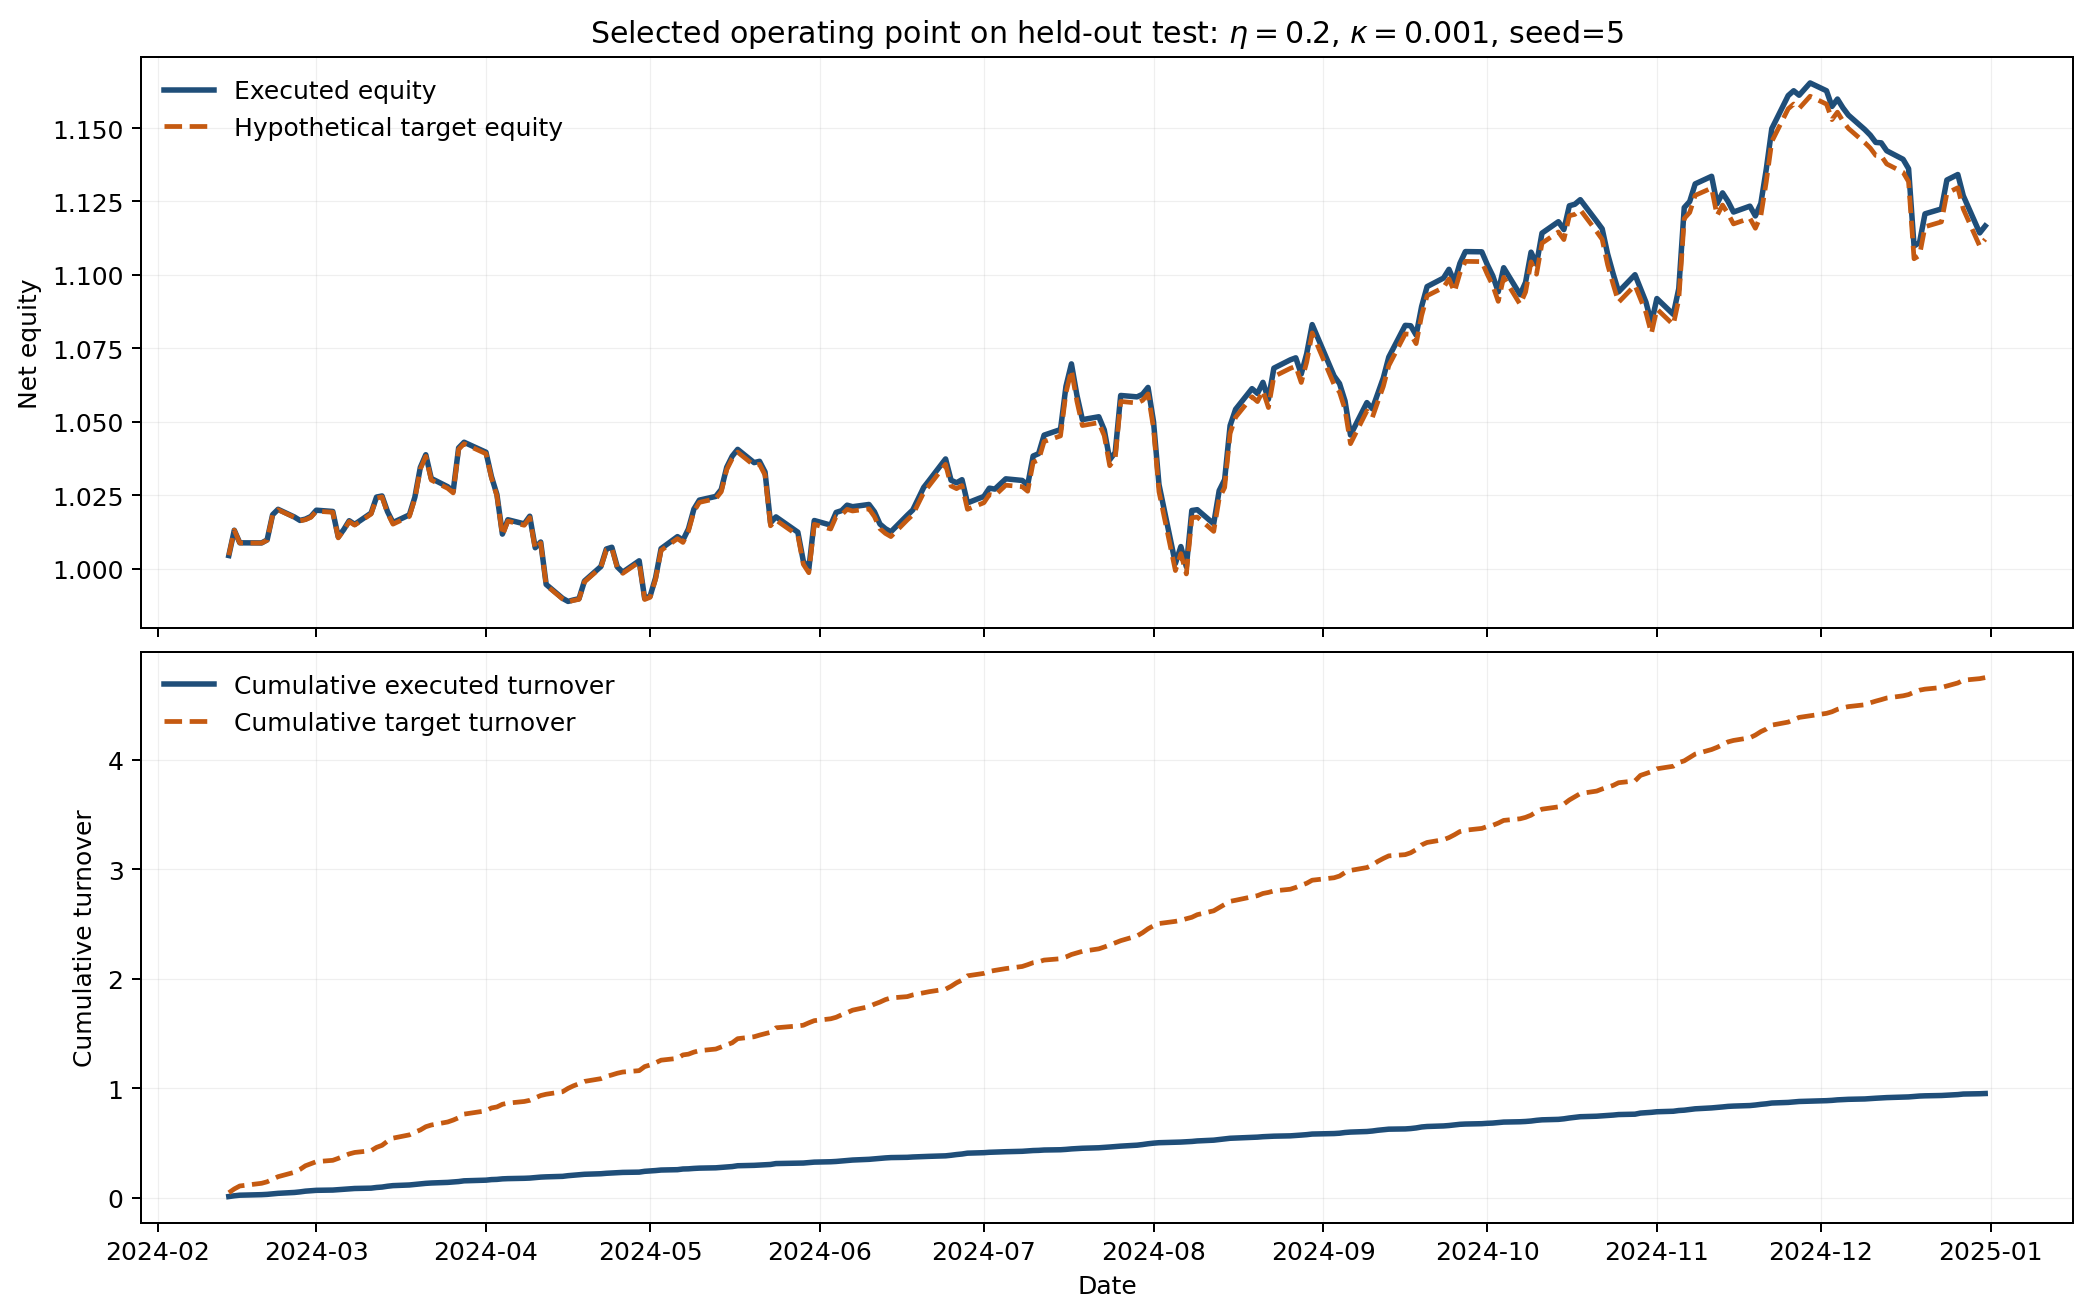
\includegraphics[width=0.95\textwidth]{fig_misalignment.png}
\caption{Representative held-out trace for the validation-selected operating point on the 2024--2025 test window at $\eta=0.2$, $\kappa=10^{-3}$, seed 5. The top panel shows executed net equity and hypothetical target net equity, where the target path is the immediate move to the target portfolio used only for diagnostics. The bottom panel shows cumulative executed and target turnover. The representative seed is the selected-arm run whose held-out net Sharpe is closest to the median selected-arm net Sharpe across the 10 paired seeds at $\kappa=10^{-3}$.}
\label{fig:misalign}
\end{figure*}

\begin{figure*}[t]
\centering
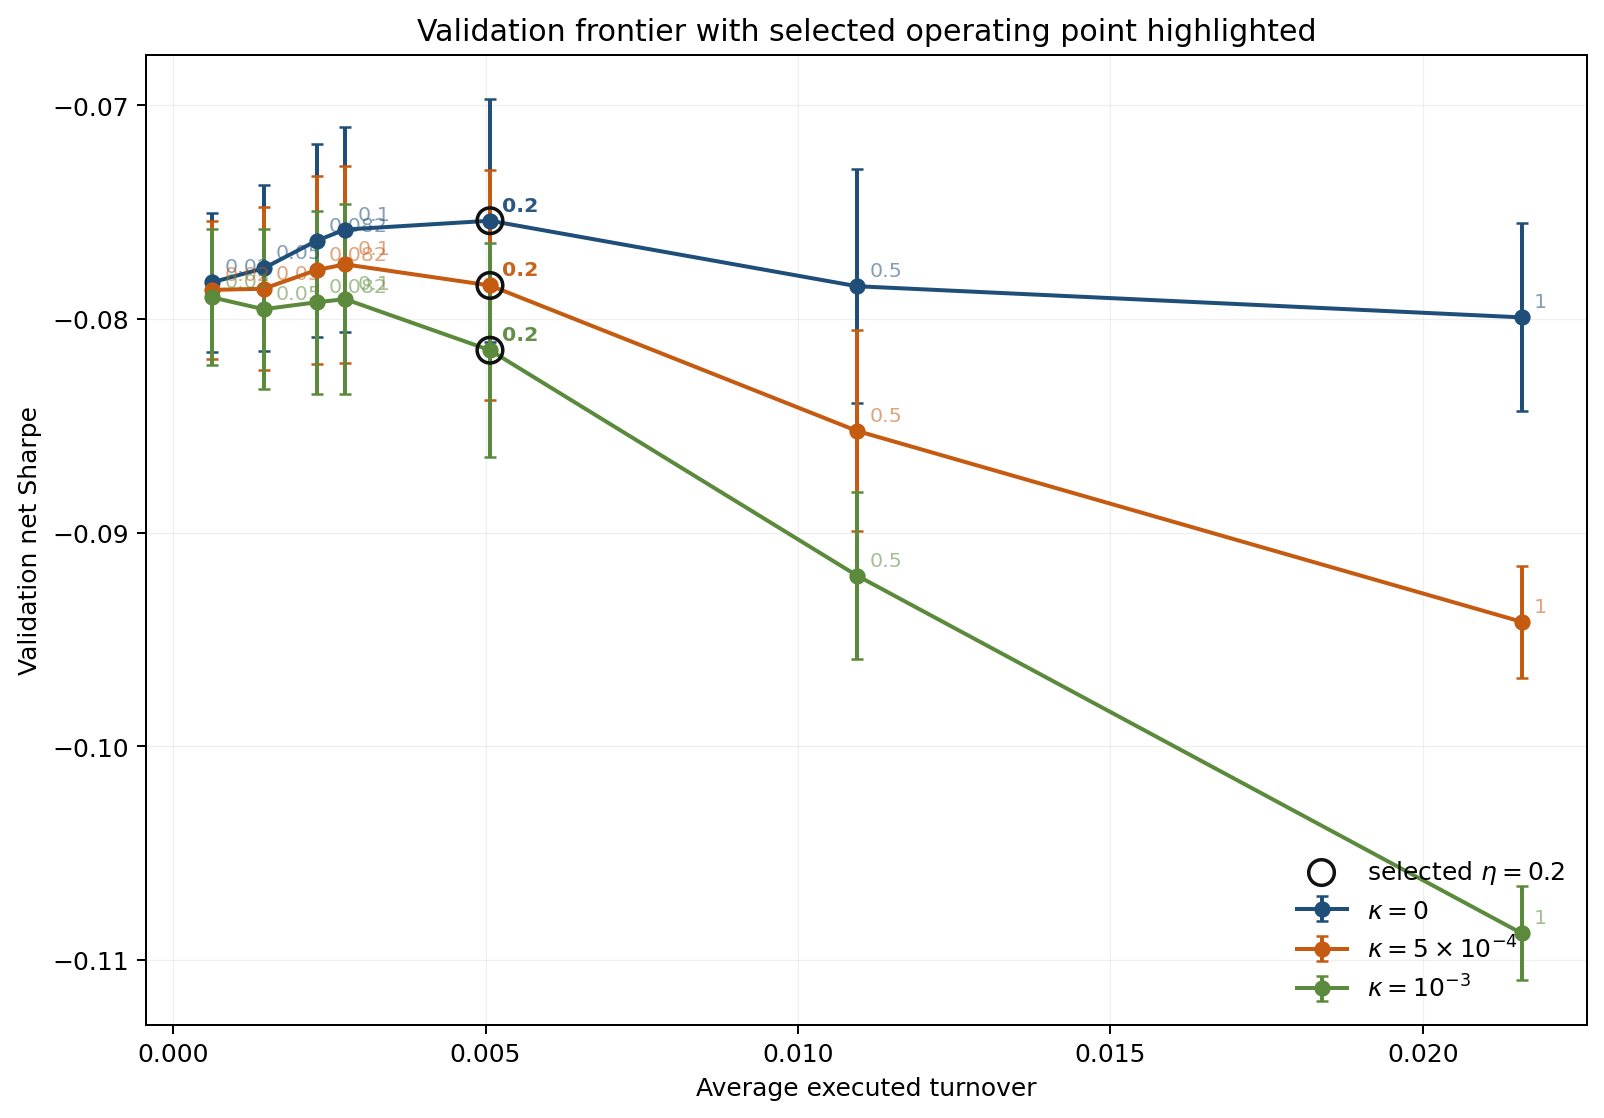
\includegraphics[width=0.95\textwidth]{fig_frontier.png}
\caption{Validation frontier on 2022--2023 under the fixed $\eta$ grid. Each colored line corresponds to one transaction-cost regime $\kappa\in\{0,5\times10^{-4},10^{-3}\}$, and each labeled point is one $\eta$ value. Horizontal position is the median executed turnover across the 10 validation seeds, vertical position is the median net Sharpe, and vertical bars show half-IQR of seedwise net Sharpe. The validation-selected operating point $\eta=0.2$ is emphasized with enlarged black-edged markers.}
\label{fig:frontier}
\end{figure*}

\begin{figure*}[t]
\centering
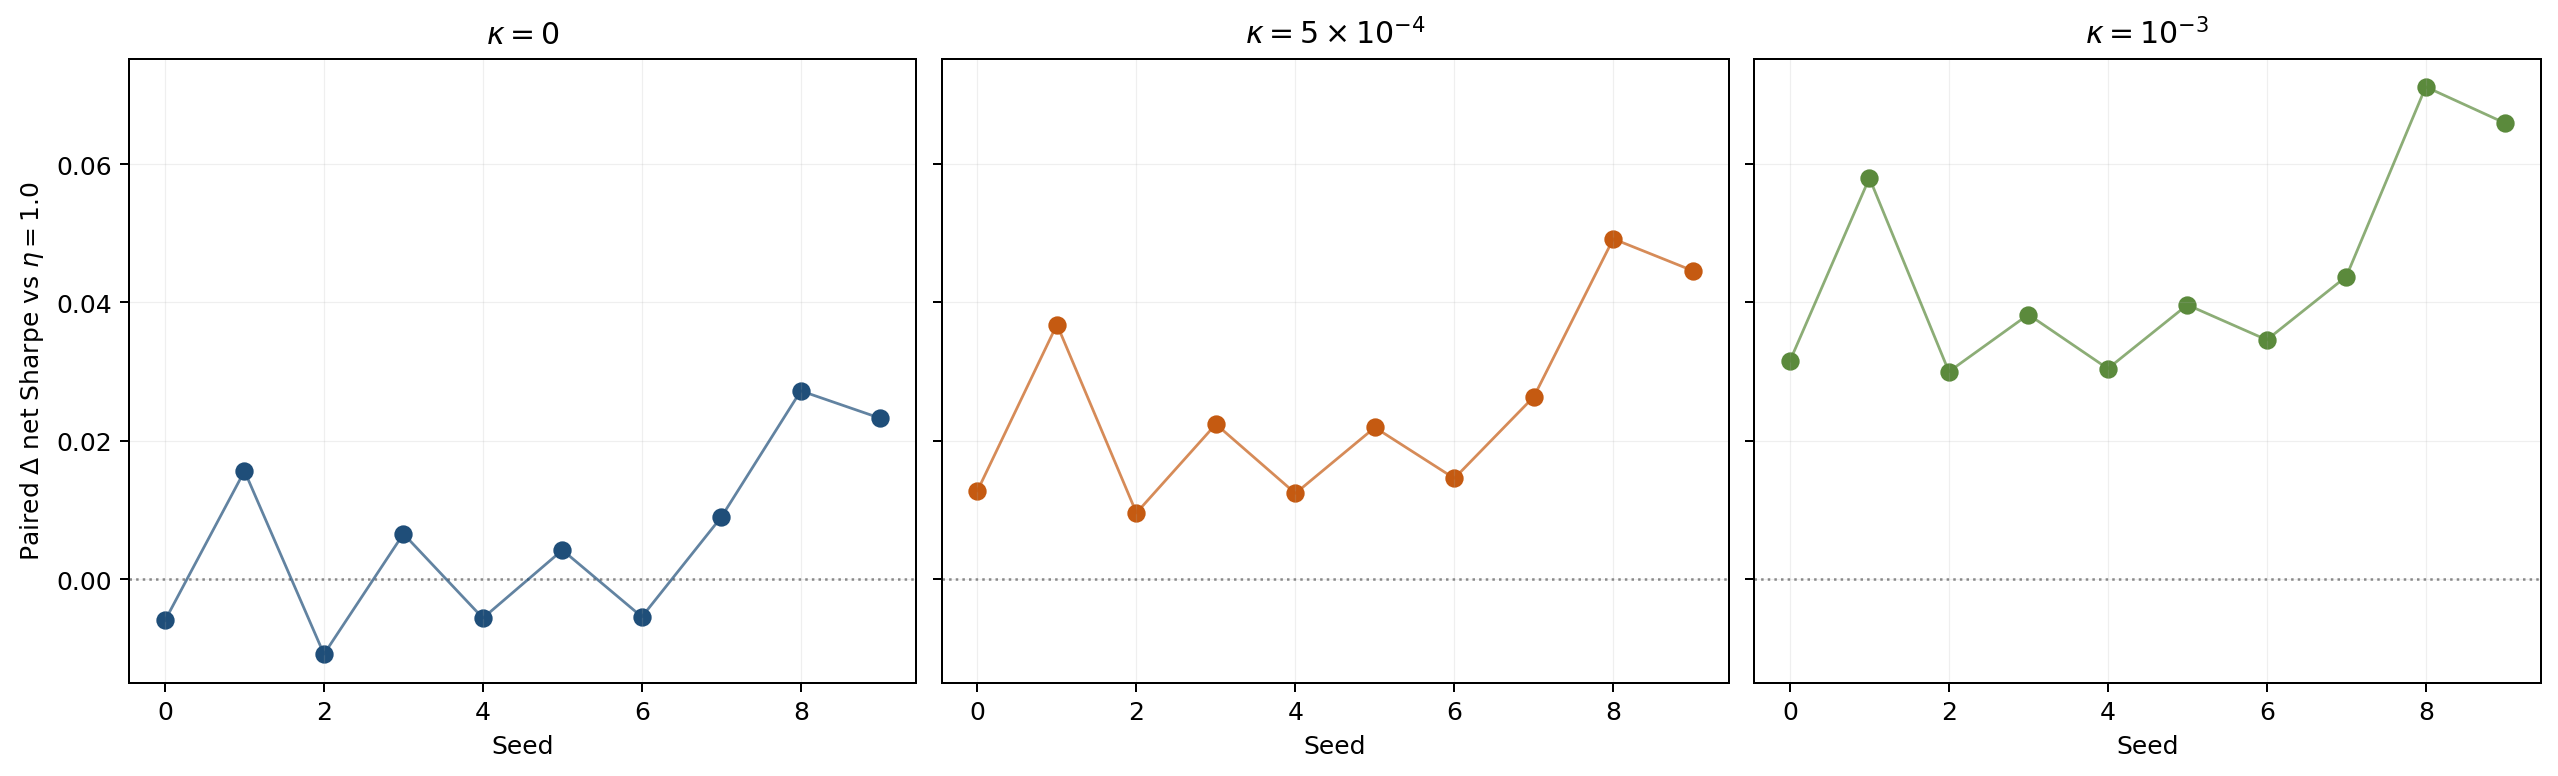
\includegraphics[width=0.90\textwidth]{fig_seed_scatter.png}
\caption{Seed-wise paired $\Delta$ net Sharpe on the 2024--2025 held-out test window for the validation-selected operating point $\eta=0.2$ relative to the immediate-execution baseline $\eta=1.0$. Each point is one seed-wise difference $\mathrm{Sharpe}_{\eta=0.2}-\mathrm{Sharpe}_{\eta=1.0}$, and the dotted horizontal line marks zero. All 10 paired seeds are positive in the two positive-cost regimes, whereas the $\kappa=0$ panel mixes positive and negative deltas.}
\label{fig:seedscatter}
\end{figure*}

% ============================================================
\section{Discussion}
\paragraph{Interpretation: realized-path stabilization, not alpha creation.}
In the present 2024--2025 test window, absolute Sharpe remains positive across both the validation-selected operating point and the immediate-execution baseline plus matched heuristic baselines. The evidence therefore supports a stabilization interpretation: execution-aware control improves risk-adjusted performance primarily by reducing harmful rebalancing variance and, when $\kappaTC>0$, by reducing realized costs rather than by injecting predictive alpha. This is also why the paper is framed as a frozen-policy execution study: the observed benefit comes from changing how the learned target path is implemented and accounted for, not from showing that a different prediction model has been learned.

\paragraph{When and why does execution help most?}
The present results point to three clear mechanisms:
\begin{itemize}[leftmargin=*,itemsep=1pt]
\item Benefits are strongest when transaction costs are non-zero. For the validation-selected operating point $\eta=0.2$, paired median net Sharpe gains are $+0.0222$ at $\kappa=5\times10^{-4}$ and $+0.0390$ at $\kappa=10^{-3}$, with $10/10$ seed wins in both regimes.
\item Turnover reduction is large even for the selected interior operating point: median executed turnover falls from $0.02184$ at $\eta=1.0$ to $0.00499$ at $\eta=0.2$, while the turnover ratio $\overline{\TOtgt}/\overline{\TOexec}$ is about $5.0$ and median tracking error remains around $0.00474$.
\item The practical trade-off is therefore not ``smaller $\eta$ is always better,'' but whether reduced realized costs outweigh additional tracking drift and reduced raw growth. The locked validation-first protocol selects an interior value $\eta=0.2$, not the smallest $\eta$ on the grid, which is consistent with this compromise interpretation.
\end{itemize}

\paragraph{How should the external-baseline result be read?}
The matched heuristic comparison is strong in net Sharpe and turnover efficiency, but not in absolute return dominance. On the 2024--2025 test window, the selected operating point has higher net Sharpe than all five matched heuristics under all reported cost regimes, while its CAGR is not uniformly higher. This asymmetry is informative: the present contribution is about cost-aligned realized-path control, not about universally maximizing raw terminal growth. In other words, the selected operating point looks stronger as a risk-adjusted execution policy than as a pure return-maximization rule.

\paragraph{Limitations.}
The limitation structure mirrors the contribution structure. The paper contributes (i) cost-aligned executed-path accounting, (ii) a fixed-$\eta$ execution mapping analysis, and (iii) a frozen-policy empirical study; correspondingly, the current evidence is limited by the market abstraction used for accounting, the fixed-timescale design, and the absence of retraining comparisons.
\begin{itemize}[leftmargin=*,itemsep=1pt]
\item The executed-path accounting contribution is established under a daily close-to-close abstraction, a fixed Dow30-style universe snapshot, and a no-cash long-only simplex; those choices make the accounting object clear, but they also limit market realism and leave survivorship-related bias unresolved.
\item The execution-mapping contribution is established only for fixed $\eta$ schedules. Adaptive execution schedules, richer control laws, and cash-aware execution are left for future work.
\item The frozen-policy empirical contribution isolates execution effects under one frozen control model, but it does not yet test whether execution-aware retraining outperforms immediate-execution training.
\item The matched baseline comparison now uses aligned accounting conventions, but the external baseline set is still small. Stronger classical references and additional robust heuristics would further tighten the empirical positioning.
\end{itemize}

% ============================================================
\section{Conclusion}
We formulated execution-aware portfolio RL by separating target and executed portfolios and enforcing execution-based reward and cost accounting. The present empirical contribution is intentionally narrow: a frozen-policy execution study with a locked validation-first protocol in which the $\eta$ grid is fixed \emph{a priori}, $\eta$ is selected on validation only, and the test window is reserved for final held-out evaluation of the selected operating point and matched comparators. In the rebuilt run, the validation-selected operating point is $\eta=0.2$.

On the held-out 2024--2025 test window, the selected operating point cuts median executed turnover from $0.02184$ to $0.00499$ and improves paired median net Sharpe by $+0.0222$ at $\kappa=5\times10^{-4}$ and $+0.0390$ at $\kappa=10^{-3}$ relative to immediate execution, with $10/10$ seed wins in both positive-cost regimes. Against matched heuristic baselines, the selected operating point is competitive in net Sharpe and turnover efficiency, though not uniformly superior in CAGR. At $\kappa=0$, the evidence is consistent with stabilization of the realized trading path but remains too weak to support a strong claim that execution-aware training itself improves learning. The safe main claim is therefore that cost-aligned execution control matters, that a validation-selected operating point can transfer to held-out test data, and that this operating point can be competitive on risk-adjusted metrics without dominating raw growth.

Future work should focus on explicit training-time alignment comparisons, stronger external baselines, and adaptive execution schedules on top of this locked evaluation protocol.

% ============================================================
\appendix
\section{Reproducibility Checklist}
\label{app:repro}
\begin{itemize}[leftmargin=*,itemsep=1pt]
\item Paired-seed evaluation across all arms.
\item Per-run config archiving and command logging.
\item Environment signature files to detect drift.
\item Automated aggregation outputs (tables/figures) generated from stored traces.
\item Hard-locked core definitions: \eqref{eq:exec_update}--\eqref{eq:reward}.
\end{itemize}

\section{Data and Protocol Clarifications}
\label{app:data_protocol}
\subsection{Fixed universe, cache, and adjusted-close data}
The paper rebuild uses a cache-only paper-mode snapshot built from daily yfinance data with adjusted close prices. Adjusted close is used so that stock splits and dividend adjustments are reflected in the return series rather than treated as spurious price jumps. The processed cache for the locked run is the fixed directory \texttt{data/processed\_u27}, and the frozen training config uses a fixed-list universe with 27 assets:

\begin{quote}
\small\ttfamily
AAPL, AMGN, AXP, BA, CAT, CRM, CSCO, CVX, DIS, GS, HD, HON, IBM, INTC, JNJ, JPM, KO, MCD, MMM, MRK, MSFT, NKE, PG, UNH, V, VZ, WMT
\end{quote}
This is a reproducible fixed snapshot, not a historical point-in-time Dow30 constituent reconstruction. Accordingly, the empirical protocol should be interpreted as a controlled benchmark study with survivorship-related limitations, not as a deployment-grade backtest free of constituent-selection bias.

\subsection{Decision timing and return interval}
The backtest uses a close-to-close convention. At decision time $t$:
\begin{enumerate}[leftmargin=*,itemsep=1pt]
\item the state $s_t$ is built only from information available up to close $t$,
\item the policy outputs the target portfolio $\wtgt_t$,
\item the execution controller forms the executed portfolio $\wexec_t$ via \eqref{eq:exec_update},
\item transaction cost is charged on executed turnover $\TOexec_t$ via \eqref{eq:cost_exec},
\item the realized return applied to the portfolio is the next-period close-to-close return over $(t,t+1]$.
\end{enumerate}
Thus the paper uses the convention ``decide at close $t$, then hold $\wexec_t$ over $(t,t+1]$.'' This ordering is important because both return realization and cost accounting are attached to the executed portfolio rather than to the raw target action.

\subsection{Frozen split and model-selection lock}
The locked rebuild materializes the experiment configuration before evaluation. The train, validation, and held-out test windows are frozen as 2010--2021, 2022--2023, and 2024--2025, respectively. The selected signal snapshot is also frozen before validation and test evaluation; in the rebuilt run, the frozen signal list is \texttt{reversal\_5d} and \texttt{short\_term\_reversal}. The $\eta$ grid is fixed \emph{a priori}, validation selects one operating point, and the test window is then used only for final evaluation of that selected operating point and matched comparators. Internal forward checks for 2026 were used only for engineering sanity and are not included in the paper tables or in $\eta$ selection.

\subsection{Constraint set and omitted assets}
All experiments use a long-only, fully invested simplex. In particular, portfolio weights are constrained to be non-negative and to sum to one each period. The present study does not include an explicit cash asset, leverage, or short positions. This means that the execution controller studies the effect of partial adjustment within a risky-asset simplex only. The no-cash design is intentional for interpretability, but it also limits the strategy class and should be read as a scope restriction rather than as a claim about the best practical trading interface.

\subsection{Backtest scope limitations}
The protocol is designed to be reproducible and internally consistent, but its scope remains limited in several ways:
\begin{itemize}[leftmargin=*,itemsep=1pt]
\item fixed-universe Dow30 snapshot rather than point-in-time constituent reconstruction,
\item no explicit cash asset,
\item long-only fully invested simplex,
\item daily close-to-close execution abstraction rather than intraday microstructure modeling,
\item frozen-policy empirical scope rather than a full retraining comparison.
\end{itemize}
These limitations do not invalidate the execution-accounting contribution, but they do bound the external claims that should be made from the current experiments.

\section{Implementation Details}
\label{app:implementation_details}
\begin{itemize}[leftmargin=*,itemsep=1pt]
\item Data source and cache: a yfinance adjusted-close snapshot is materialized once and then reused in cache-only paper mode for training and evaluation.
\item Universe treatment: the present draft uses a fixed Dow30 ticker set rather than a point-in-time constituent reconstruction.
\item Timing convention: features at time $t$ use information available by close $t$, and realized returns are applied over the next close-to-close interval $(t,t+1]$.
\item Anti-lookahead: observations use rolling historical returns, contemporaneous volatility estimates, and previous executed weights only.
\end{itemize}

% ============================================================
\begin{thebibliography}{99}
\bibitem{markowitz1952}
H. Markowitz, ``Portfolio Selection,'' \emph{The Journal of Finance}, 1952.

\bibitem{merton1973}
R. C. Merton, ``An Intertemporal Capital Asset Pricing Model,'' \emph{Econometrica}, 1973.

\bibitem{moody1998}
J. Moody and M. Saffell, ``Learning to Trade via Direct Reinforcement,'' \emph{IEEE Transactions on Neural Networks}, 1998.

\bibitem{jiang2017}
Z. Jiang, D. Xu, and J. Liang, ``A Deep Reinforcement Learning Framework for the Financial Portfolio Management Problem,'' \emph{CoRR}, abs/1706.10059, 2017.

\bibitem{ye2020}
Y. Ye, H. Pei, B. Wang, P.-Y. Chen, Y. Zhu, J. Xiao, and B. Li, ``Reinforcement-Learning Based Portfolio Management with Augmented Asset Movement Prediction States,'' \emph{Proceedings of the AAAI Conference on Artificial Intelligence}, 34(1):1112--1119, 2020.

\bibitem{lien2023}
Y.-H. Lien, Y.-K. Li, and Y.-S. Wang, ``Contrastive Learning and Reward Smoothing for Deep Portfolio Management,'' \emph{Proceedings of the Thirty-Second International Joint Conference on Artificial Intelligence (IJCAI-23)}, pp. 3966--3974, 2023.

\bibitem{lobo2007}
M. Lobo, M. Fazel, and S. Boyd, ``Portfolio Optimization with Linear and Fixed Transaction Costs,'' \emph{Annals of Operations Research}, 152(1):341--365, 2007.

\bibitem{garleanu2013}
N. G\^arleanu and L. H. Pedersen, ``Dynamic Trading with Predictable Returns and Transaction Costs,'' \emph{The Journal of Finance}, 68(6):2309--2340, 2013.

\bibitem{almgren2000}
R. Almgren and N. Chriss, ``Optimal Execution of Portfolio Transactions,'' \emph{Journal of Risk}, 3(2):5--39, 2000.

\bibitem{shen2020}
Q. Shen, Y. Li, H. Jiang, Z. Wang, and T. Zhao, ``Deep Reinforcement Learning with Robust and Smooth Policy,'' \emph{Proceedings of the 37th International Conference on Machine Learning}, \emph{PMLR} 119:8707--8718, 2020.

\bibitem{mysore2021}
S. Mysore, B. Mabsout, R. Mancuso, and K. Saenko, ``Regularizing Action Policies for Smooth Control with Reinforcement Learning,'' \emph{Proceedings of the IEEE International Conference on Robotics and Automation (ICRA)}, pp. 1810--1816, 2021.
\end{thebibliography}

\end{document}
